Este capítulo apresentará a fundamentação teórica utilizada neste trabalho, abordando os temas mais pertinentes, como Sistemas Embarcados, Robótica, Reconhecimento de padrões, e Modelagem de sistemas.

% ==================================================
\section{Sistemas Embarcados}
\label{sec:embarcados}
% ==================================================

Sistemas computacionais estão presentes em diversos produtos desde computadores pessoais e \textit{laptops}, até utensílios domésticos. São conhecidos como sistemas embarcados (SE) os sistemas computacionais que fazem parte de um dispositivo eletrônico maior, não representando sua totalidade, mas oferecendo recursos computacionais específicos para o seu funcionamento \cite{vahid:2002}.

Também pode-se definir um SE como um sistema computacional de propósito específico, e que não assume vários papéis de acordo com a necessidade do usuário, apenas realiza tarefas predeterminadas, em contraste a um computador pessoal \cite{heath:2002}. Isto é, são sistemas eletrônicos projetados para funções específicas dentro de um dispositivo maior, que pode controlar o meio físico e permite sua interação com o usuário.

Algumas características de sistemas embarcados, segundo \citeonline{schlett:1998}, são restrições específicas como de custo de produção ou de consumo de energia, que é o caso de dispositivos móveis, por exemplo, pois dependem de uma bateria para funcionar. \citeonline{vahid:2002} citam também como exemplo de sistema embarcado uma câmera fotográfica digital, pois tem um propósito específico (capturar e processar fotografias) e tem restrições de tamanho, custo, e consumo de energia.

Uma outra restrição comum que pode ser pertinente a um SE é de tempo. Alguns sistemas precisam necessariamente realizar certas operações dentro de um tempo esperado, correndo o risco de não desempenhar seu papel caso isso falhe, sendo conhecidos como sistemas em tempo real. Por exemplo, um sistema de controle de velocidade de cruzeiro de um automóvel precisa monitorar a velocidade, aceleração e desaceleração do veículo em tempo real, e qualquer atraso é considerado uma falha do sistema \cite{vahid:2002}.

\todo[inline]{\textbf{Falar um pouco mais de tempo real} \textit{e qual é a relação com a robótica}}
Sistemas robóticos, do ponto de vista de arquitetura, dependem de interação com ambientes dinâmicos e incertos, o que exige controle em tempo real dos sensores e atuadores, com suporte a concorrência e reagindo rapidamente a situações excepcionais \cite{siciliano:2008springer}.

% ==================================================
\subsection{Microcontroladores versus Microprocessadores}
% ==================================================

Microcontroladores são processadores com vários componentes integrados, como RAM, uma memória de programa e interfaces de entrada e saída \cite{white:2011}. Esses componentes surgiram como um substituto para circuitos lógicos discretos, por serem mais facilmente programáveis e proporcionarem uma funcionalidade maior \cite{heath:2002}. Além disso, segundo \citeonline{marwedel:2010}, os processadores em sistemas embarcados são geralmente microcontroladores, por serem simples e fáceis de usar.

A distinção entre microprocessadores e microcontroladores, contudo, não é tão trivial: \citeonline{schlett:1998} afirma que, de forma simplificada, é comum diferenciá-los tendo como parâmetro seu desempenho, considerando dispositivos de $8$ e $16$-bit como microcontroladores. Mas também existem outros critérios a se considerar, como sua finalidade e suas possíveis restrições de energia, ou a necessidade de integração com vários componentes periféricos.

Os microprocessadores, por sua vez, não contam com RAM e ROM integradas e contém apenas cache. Este tipo de processador é encontrado nos computadores pessoais e costumam ter um desempenho aprimorado em relação aos microcontroladores. Por esse motivo, alguns sistemas embarcados passaram a usar microprocessadores também, pois alguns dispositivos como \textit{video games} portáteis passaram a exigir maior capacidade de processamento. No entanto, estes microprocessadores embarcados ainda costumam ter restrições como de energia, custo, etc \cite{schlett:1998}.

\todo[inline]{Apresentar exemplo de Microcontrolador, exemplo Arduino suas funções e pinagens}

\todo[inline]{Apresentar exemplo de Microprocessador, exemplo Galileo suas funções e pinagens}

% ==================================================
\subsection{IoT: Internet das Coisas}
% ==================================================
Com a constante evolução e a ubiquidade da Internet, começam a surgir objetos conectados, transformando dispositivos que já faziam parte do cotidiano em algo que possa ser autônomo e inteligente \cite{kopetz:2011}.  Segundo \citeonline{xia:2012}, o termo ``Internet das Coisas'' (IoT)  não refere-se apenas à existência destes dispositivos inteligentes, mas à interconexão dos objetos do cotidiano através de sistemas embarcados, proporcionando assim ambientes em que os dispositivos se comunicam entre si e também com seres humanos de forma inteligente.

Para \citeonline{gubbi:2013iot}, a visão completa da IoT se dará através de sensores e atuadores ubíquos, escondidos do usuário, atuando de forma independente. A ideia de computação ubíqua, também conhecida como pervasiva \cite{satyanarayanan:2001pervasive}, está bem relacionada com a IoT e se refere a um mundo repleto de sensores, atuadores e sistemas computacionais integrados nos objetos do dia-a-dia \cite{gubbi:2013iot}.

Um exemplo de objeto inteligente na IoT, segundo \citeonline{kopetz:2011}, é uma geladeira que mantém registro da validade e disponibilidade dos itens contidos, e faz pedidos automaticamente ao supermercado mais próximo dos produtos em falta.

\todo[inline]{Apresentar um exemplo de IoT com robótica}

% ==================================================
\section{Robótica e suas Aplicações}
\label{sec:robotica}
% ==================================================

A robótica é uma área que busca sintetizar atividades humanas através do uso de mecanismos, sensores, atuadores e computadores. É comum que pesquisas neste campo sejam feitas por pesquisadores de outras áreas, servindo como meio para diversos fins \cite{craig:2005}. Sistemas embarcados são tradicionalmente usados na área da robótica, relacionando-se aos aspectos mecânicos \cite{marwedel:2010}. \citeonline{craig:2005} divide a robótica em quatro grandes áreas: manipulação mecânica, locomoção, visão computacional e inteligência artificial.

\todo[inline]{Apresentar um exemplo de uso na indústria com uma imagem}

A robótica de reabilitação consiste em auxiliar pessoas com dificuldades motoras ou cognitivas por meio de sistemas como próteses robóticas e outros tipos de dispositivos, como os aparelhos de auxílio na restauração do andar de pacientes na \autoref{fig:rehab_gait} \cite{siciliano:2008springer}. Neste contexto, a robótica tem sido aplicada para aprimorar a mobilidade de pessoas com membros amputados, através de próteses ativas, que podem permitir, por exemplo, uma caminhada mais natural do que uma prótese passiva comum \cite{dedic:2011}. Alguns projetos deste tipo, além deste trabalho, serão discutidos no \autoref{ch:correlatos}.

\todo{Trocar por foto de prótese}\begin{figure}[ht]
	\caption{\label{fig:rehab_gait}Exemplos de robôs de reabilitação de andar}
	\begin{center}
	    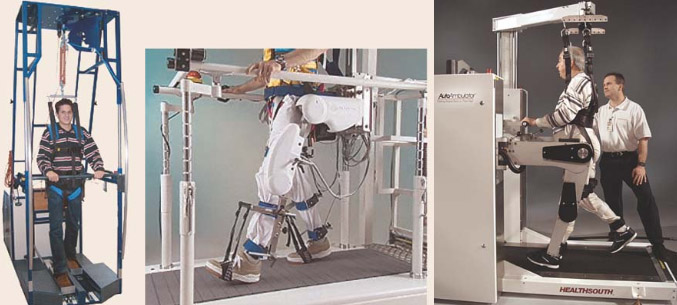
\includegraphics[width=0.9\textwidth]{resources/robotics_rehab_1}
	\end{center}
	\legend{Fonte: \citeonline[p.1232]{siciliano:2008springer}}
\end{figure}

\todo[inline]{Apresentar e descrever sensores e atuadores utilizados na robótica}

\todo[inline]{Apresentar detalhes sobre mecânica na robotica - ver http://www.leomar.com.br/brinquedos/images/stories/manuais/laboratorio/guia\%20de\%20robotica.pdf}

\todo[inline]{Falar sobre as platormas de desenvolvimento para robótica, como Lego Mindstorm - ver http://livros01.livrosgratis.com.br/cp115615.pdf}

% \section{Eletromiografia: Geração de Dados}
% \label{sec:emg}
% A eletromiografia (EMG) é uma técnica que consiste em monitorar atividade neuromuscular, sendo possível assim detectar os potenciais de ação através desta leitura \cite{deluca:1979}. Em teoria, isto significa que, a partir do eletromiograma, é possível identificar a intenção de uma pessoa ao realizar uma atividade motora.

% A leitura dos sinais eletromiográficos pode ser feita de diferentes formas: por profundidade ou por superfície. O primeiro método consiste em inserir uma agulha que atinja o músculo desejado, permitindo a captação dos sinais; já a eletromiografia por superfície (sEMG) utiliza apenas um conjunto eletrodos sobre a pele, na região do músculo desejado \cite{deluca:1979}

% Com os dados extraídos a partir da EMG, é possível que se desenvolva próteses controláveis baseadas no reconhecimento de padrões e classificação dos dados eletromiográficos a partir dos músculos intactos \cite{park:1998}.

% No caso da sEMG, a superfície da pele tem diversos sinais com amplitude maior que da eletromiografia. Isso torna necessário o uso de uma configuração diferencial: analisa-se dois sinais de duas superfícies diferentes para que sejam subtraídos os sinais a fim de se obter a informação desejada. Dessa forma, as áreas de detecção e a distância entre elas são fatores importantes, pois afetam a amplitude e frequência do sinal \cite{deluca:1997}.

% \textcolor{red}{TODO!}\todo{Inserir imagem com posicionamento de eletrodos e exemplo de leitura dos sinais.}

% ==================================================
\section{Reconhecimento de Padrões}
\label{sec:patternrec}
% ==================================================

O reconhecimento de padrões é um campo que busca encontrar padrões em conjuntos de dados, com finalidade em diversas áreas, e vem sendo desenvolvido ao lado de Aprendizado de Máquina\todo{Adicionar referência.}\ no decorrer dos anos. Com isto, a intenção é usar algoritmos computacionais no intuito de descobrir automaticamente regularidades em dados, possibilitando, por exemplo, a classificação de tais dados \cite{bishop:2006}.

Os dados extraídos de sensores podem ser usados para classificação a partir do reconhecimento de padrões. Esta seção abordará o aprendizado de máquina e alguns \textit{frameworks} que podem ser usados na classificação dos movimentos a partir desses dados.

% ==================================================
\subsection{Aprendizado de máquina}
\label{sec:ml}
% ==================================================

O aprendizado de máquina é importante quando não é possível determinar todos cenários possíveis de um sistema previamente, ou quando se deseja que este se adapte ao ambiente por conta própria. Também há o caso de ser impossível uma pessoa programar uma solução por conta própria, por exemplo: humanos conseguem reconhecer faces muito bem, mas não são capazes de desenvolver um programa que realize esta tarefa, sem usar algoritmos de aprendizagem \cite{russell:2010}.

Existem três principais formas de aprendizagem que são determinadas a partir do tipo de \textit{feedback} dado ao algoritmo. No \textbf{aprendizado não supervisionado}, o agente aprende os padrões da entrada mesmo sem ter nenhum tipo de \textit{feedback}. Agrupamento (ou \textit{clustering}) é o tipo de aprendizagem não supervisionada mais comum, em que se detecta grupos a partir de exemplos de entrada. O \textbf{aprendizado por reforço} consiste em aprender baseado em um \textit{feedback} positivo ou negativo do resultado do algoritmo, indicando se algo de errado foi feito. Dessa forma, decide-se que ações pode ter ocasionado um resultado indesejado \cite{russell:2010}.

No \textbf{aprendizado supervisionado}, o agente observa pares de entrada e saída e aprende uma função que mapeia os valores de entrada para os de saída, aplicando essa função em entradas futuras. Os pares de entrada e saída são chamados de conjunto de treinamento e a função a ser encontrada é chamada de hipótese. Para medir a acurácia da hipótese, é escolhido um conjunto de teste, diferente do conjunto de treinamento. Considera-se que a hipótese é uma boa generalização se for capaz de prever o valor de saída dos exemplos de teste \cite{russell:2010}.

Quando os valores de saída são números, o problema é conhecido como \textbf{regressão}. Quando a saída é um conjunto de valores finitos, o problema de aprendizagem é chamado de \textbf{classificação}, também conhecido como classificação Booleana ou binária caso hajam apenas dois valores \cite{russell:2010}.

% \subsubsection{SVM}
Uma das técnicas mais populares de aprendizado de máquina supervisionado é a Máquina de Vetores de Suporte (SVM, em inglês), por não exigir um conhecimento prévio do domínio em que será aplicado \cite{russell:2010}.

A SVM funciona ao encontrar um hiperplano que tem a maior margem possível entre as diferentes classes \cite{hearst:1998}. Como no exemplo da figura~\ref{fig:svm_classification}, é possível ver três hiperplanos em \ref{fig:svm_classification_a} e o separador linear desejado em \ref{fig:svm_classification_b}, consistindo no hiperplano com a maior margem entre os vetores de suporte, que são os pontos circulados \cite{russell:2010}. Neste exemplo, é feita a classificação entre os círculos pretos e os brancos.

\begin{figure}[ht]
    \centering
    \caption{Classificação binária com SVM}
    \label{fig:svm_classification}
    \subfloat[Duas classes de pontos (círculos pretos e brancos) e três candidatos a separadores lineares. \label{fig:svm_classification_a}]
        {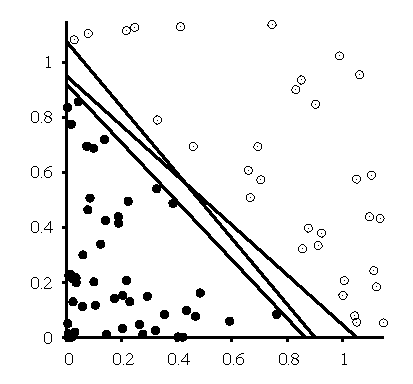
\includegraphics[width=0.4\textwidth]{resources/svm_russel_classification_a}}
        \hspace{0.2cm}
    \subfloat[O separador com maior margem (linha escura) no ponto médio da margem (entre as linhas tracejadas). Os vetores de suporte (pontos circulados) são os mais próximos ao separador. \label{fig:svm_classification_b}]
        {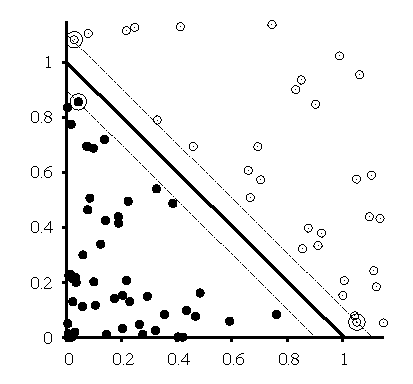
\includegraphics[width=0.4\textwidth]{resources/svm_russel_classification_b}}
        \legend{Fonte: Adaptado de \citeonline[p. 745]{russell:2010}}
\end{figure}
%\textcolor{red}{Testes figura~\ref{fig:svm_classification}, e as figuras~\ref{fig:svm_classification_a}~e~\ref{fig:svm_classification_b}.}

% ==================================================
\subsection{Ferramentas para aprendizado de máquina}
\label{sec:ml_tools}
% ==================================================

Dada a complexidade de algoritmos de aprendizado de máquina, e visando auxiliar na produção de soluções em diversas áreas, estão disponíveis diferentes ferramentas de desenvolvimento, como scikit-learn \cite{pedregosa:2011} e Tensorflow \cite{abadi:2015}. Algumas destas ferramentas serão abordadas nas próximas seções.

% ==================================================
\subsubsection{Scikit-learn}
\label{sec:ml_sklearn}
% ==================================================

O scikit-learn\footnote{\href{http://scikit-learn.org/}{<http://scikit-learn.org/>}} é um módulo para a linguagem Python que integra uma alta gama de algoritmos de aprendizado de máquina, tanto supervisionados quanto não supervisionados, como SVM, KNN, e K-Means\todo{Adicionar referências das técnicas?}, e permite a comparação fácil de diversos métodos em uma aplicação \cite{pedregosa:2011}.

Segundo \citeonline{pedregosa:2011}, o scikit-learn aproveita o alto nível da linguagem Python para manter a facilidade de uso do \textit{framework}, tornando-o utilizável por não especialistas da indústria de software e em campos além da ciência da computação. Além disso, \citeonline{pedregosa:2011} garantem maior eficiência do que outras ferramentas semelhantes em Python, pois o scikit-learn incorpora código compilado. A \autoref{fig:sklearn_svm} demonstra exemplos de classificação em SVM, com diferentes características, feitos com o scikit-learn.

\begin{figure}[ht]
	\caption{\label{fig:sklearn_svm}Exemplo de classificação de dados utilizando scikit-learn}
	\begin{center}
	    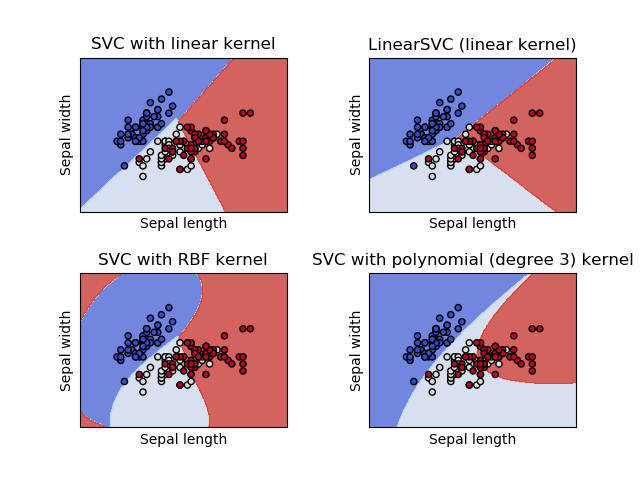
\includegraphics[width=0.8\textwidth]{resources/sklearn_iris_svm.png}
	\end{center}
	\legend{Fonte: \href{http://scikit-learn.org/stable/modules/svm.html\#classification}{<http://scikit-learn.org/stable/modules/svm.html\#classification>} \textcolor{red}{Verificar referência}}
\end{figure}

%\todo[inline]{Apresentar um exemplo de utilização da ferramenta, pode ser um trecho do próprio site}

% ==================================================
\subsubsection{TensorFlow}
\label{sec:ml_tf}
% ==================================================

TensorFlow\footnote{\href{http://tensorflow.org/}{<http://tensorflow.org/>}} é um sistema para algoritmos de aprendizado de máquina que funciona em diversos sistemas diferentes de forma flexível, sem exigir grandes alterações em uma variedade de sistemas heterogêneos \cite{abadi:2016}. É uma ferramenta bastante popular, e oferece classificação utilizando técnicas como Redes Neurais Convolutivas (CNN) e SoftMax \cite{ertram:2017}.

\todo[inline]{Ampliar esta seção está bem rasa, sugiro falar sobre as técnicas que são usadas na tool, como RNN pre-treinadas. Mencionar quem usa esta \textit{tool} e onde.}

\todo[inline]{Apresentar um exemplo de utilização da ferramenta, pode ser um trecho do próprio site}


% ==================================================
\section{Modelagem e validação de sistemas}
\label{sec:modelosformais}
% ==================================================

Sistemas embarcados são muitas vezes usados em situações críticas, em que segurança e confiabilidade são critérios muito importantes, pois podem oferecer risco à vida\todo{Apresentar exemplo}. O uso de modelos formais, como redes de Petri \cite{peterson:1981}, para descrever o comportamento do sistema antes que este seja desenvolvido e é uma forma de se aproximar da melhor confiabilidade, pois esses modelos podem ser validados automaticamente \cite{edwards:1997}.

% ==================================================
\subsection{Diagrama de sequência}
% ==================================================
Uma forma de detalhar as especificações iniciais do design do sistema é através do diagrama de sequência, que é um modelo especificado pela UML\todo{Falar um pouco sobre UML}. Este diagrama indica a troca de mensagens sequencial entre os diversos componentes de um sistema. Na figura~\ref{fig:seq_chart}, pode-se ver um exemplo de um atendedor telefônico automático. A dimensão vertical neste exemplo representa a sequência, e a horizontal representa cada componente de comunicação~\cite{marwedel:2010}.

\begin{figure}[!ht]
	\caption{\label{fig:seq_chart}Exemplo de diagrama de sequência em UML}
	\begin{center}
	    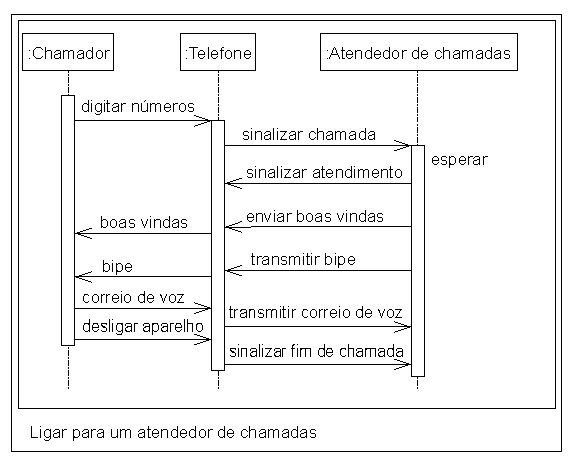
\includegraphics[width=0.8\textwidth]{resources/seq_chart_marwedel_1}
	\end{center}
	\legend{Fonte: Adaptado de \citeonline[p. 37]{marwedel:2010}}
\end{figure}

As linhas tracejadas representam as ``linhas da vida'', e as mensagens são ordenadas em sequência ao longo dessas linhas. Caixas sobre as linhas da vida representam controle ativo do componente correspondente. No exemplo da figura~\ref{fig:seq_chart}, as setas denotam mensagens assíncronas, e pode-se notar que a máquina espera o usuário atender o telefone. Caso isso não ocorra, a própria máquina atende e envia as boas vindas para o autor da chamada, que deixa uma mensagem no correio de voz~\cite{marwedel:2010}.

%Ainda segundo \citeonline{marwedel:2010}, o diagrama de sequência tem certas limitações\todo{Exemplificar quais.}\ e não é capaz de descrever ações complexas, mas é útil para uma modelagem inicial. %===> Não sei de onde eu tirei essa ideia!

% ==================================================
\subsection{Máquinas de Estado}
% ==================================================

A teoria dos autômatos é o estudo de dispositivos computacionais abstratos (``máquinas''), que servem de modelo para o projeto e construção de softwares, a partir de conceitos como autômatos finitos e gramáticas formais \cite{hopcroft:2001}.

Um autômato finito, também conhecido como Máquina de Estados Finita (FSM) \cite{wagner:2006}, se baseia em um conjunto finito de estados, entradas, saídas e transições entre estados. A descrição do comportamento baseado em estados é importante na modelagem de sistemas embarcados \cite{marwedel:2010}.

De acordo com \citeonline{wagner:2006}, uma FSM é uma quíntupla $\{\Sigma, S, s0, \delta, F\}$, onde:
\begin{itemize}
    \item $\Sigma$ é o alfabeto de entrada (um conjunto finito não vazio de símbolos)
    \item $S$ é um conjunto não vazio de estados
    \item $s0$ é um estado inicial, um elemento de $S$
    \item $F$ é o conjunto de estados finais, um subconjunto de $S$.
\end{itemize}

Cada estado de uma FSM representa uma informação sobre o decorrer do programa, pois o estado muda de tempos em tempos durante a execução, e todos os estados representam todas as situações possíveis em que a máquina de estados pode estar. As saídas podem depender tanto do estado atual quanto das entradas da máquina \cite{wagner:2006}.

\begin{figure}[ht]
	\caption{\label{fig:fsm}Exemplo de diagrama de estados}
	\begin{center}
	    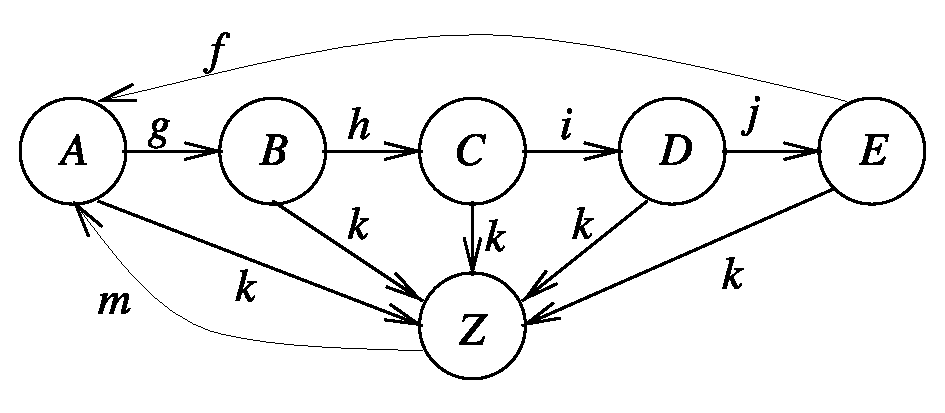
\includegraphics[width=0.6\textwidth]{resources/fsm_marwedel}
	\end{center}
	\legend{Fonte: \citeonline[p. 39]{marwedel:2010}}
\end{figure}

Um diagrama de estados como o da Figura~\ref{fig:fsm} é uma representação clássica de uma FSM. Os círculos representam estados, as arestas são transições e o rótulo das arestas são eventos de transição, que levam a máquina a mudar de estado \cite{marwedel:2010}.

A Figura~\ref{fig:fsm_2} representa um sistema de máquina de venda que aceita moedas de 5 e de 10 centavos, sendo 25 o valor esperado. O estado ``Início'' é o estado em que ainda não foi depositada uma moeda e o estado ``Fim'' quer dizer que a máquina recebeu 25 centavos. As transições representam as moedas depositadas na máquina. Em todos os estados qualquer moeda é aceita, exceto no estado ``Vinte'', em que a moeda de 10 centavos é ignorada neste exemplo por questões de simplicidade \cite{wagner:2006}.

\begin{figure}[ht]
	\caption{\label{fig:fsm_2}Diagrama de máquina de estados do contador de uma máquina de vendas}
	\begin{center}
	    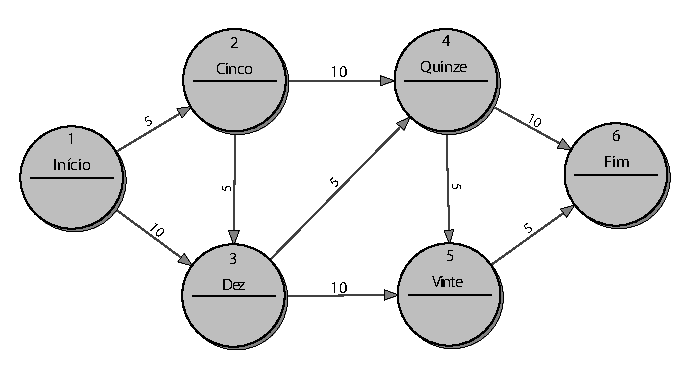
\includegraphics[width=0.8\textwidth]{resources/fsm_wagner}
	\end{center}
	\legend{Fonte: Adaptado de \citeonline[p. 68]{wagner:2006}}
\end{figure}

\todo[inline]{Descrever que propriedades podem ser validadas usando um FSM}

% ==================================================
\subsection{Redes de Petri}
% ==================================================

Uma rede de Petri é um modelo matemático de um sistema, cujo estudo pode revelar informações vitais sobre a estrutura e o comportamento do sistema modelado \cite{peterson:1981}. Segundo \citeonline{murata:1989}, as redes de Petri são uma ferramenta de modelagem matemática e gráfica, especialmente úteis para sistemas concorrentes, assíncronos, distribuídos, paralelos, não-determinísticos, e estocásticos.

A estrutura de uma rede de Petri consiste em lugares, transições, funções de entrada e funções de saída. Graficamente, sua representação é dada por um grafo direcionado, em que os lugares são representados por círculos, as transições por barras, e os arcos entre os lugares e as transições indicam entradas e saídas \cite{peterson:1981}. % $C = (P,T,I,O)

Segundo \citeonline{murata:1989}, uma rede de Petri é uma quíntupla $PN = (P, T, F, W, M_0)$, onde:

\begin{itemize}
    \item $P = \{p_1, p_2, \cdots , p_m\}$ é um conjunto finito de lugares,
    \item $T = \{t_1, t_2, \cdots, t_n\}$ é um conjunto finito de transições,
    \item $F \subseteq (P \times T) \cup (T \times P)$ é um conjunto de arcos (relação de fluxo),
    \item $W: F \to \{1,2,3,\cdots\}$ é uma função de peso,
    \item $M_0: P \to \{0,1,2,3,\cdots\}$ é a marcação inicial,
    \item $P \cap T = \emptyset$ e $P \cup T \neq \emptyset$
\end{itemize}

Uma estrutura de rede de Petri $N=(P,T,F,W)$ sem nenhuma marcação inicial é denotada por $N$, e uma rede de Petri com a marcação inicial definida é denotada por $(N,M_0)$ \cite{murata:1989}.

Cada um dos lugares é marcado com um número não negativo de \textit{tokens}. Quando os lugares têm um número positivo $k$ de \textit{tokens}, estes são representados graficamente por $k$ círculos preenchidos posicionados no interior dos círculos que representam os lugares \cite{murata:1989}, como pode ser visto nos lugares $P_1$ e $P_2$ da figura~\ref{fig:petrinet}. Uma transição é disparada de acordo com um evento determinado, desde que hajam \textit{tokens} suficientes no lugar de entrada.

\begin{figure}[ht]
	\caption{\label{fig:petrinet}Exemplo de rede de Petri com atividades paralelas}
	\begin{center}
	    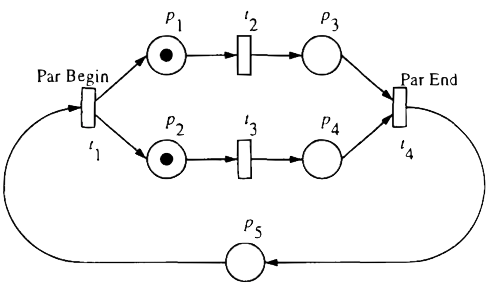
\includegraphics[width=0.6\textwidth]{resources/petri_net_murata_1}
	\end{center}
	\legend{Fonte: \citeonline[p. 545]{murata:1989}}
\end{figure}

Na \autoref{fig:petrinet} as transições $t_1$ e $t_2$ estão habilitadas, pois há \textit{tokens} suficientes nos lugares $P_1$ e $P_2$, e também são paralelas, pois suas causas são independentes. Caso uma dessas transições seja disparada, o \textit{token} no lugar de entrada é removido e um novo é produzido no lugar de saída da transição.

A partir do modelo, é possível fazer a análise da rede de Petri usando propriedades como segurança, limitação (do inglês \textit{boundedness}) e vivacidade. 
% 
Em uma rede de Petri que modela um hardware, \textit{segurança}\todo{Apresentar exemplo gráfico}\ é uma das propriedades mais importantes. Um lugar em uma rede de Petri é seguro quando nunca contém mais de um \textit{token}, e uma rede de Petri é segura se todos os lugares forem seguros. A importância desta propriedade para dispositivos de hardware se dá pelo fato de cada lugar poder ser implementado por um único \textit{flip-flop}, já que o número de um lugar pode ser apenas $0$ ou $1$ \cite{peterson:1981}.

O conceito de limitação\todo{Apresentar exemplo gráfico}\ é uma generalização da propriedade de segurança e determina o número \textit{k} de \textit{tokens} que são permitidos em cada lugar. Caso \textit{k} seja 1, então a propriedade de segurança se aplica. A limitação é essencial para especificação de hardware, e os lugares podem ser implementados com contadores \cite{peterson:1981}.

Um problema computacional comum em relação a alocação de recursos é o \textit{deadlock}, em que processos diferentes requerem recursos que estão indisponíveis e não conseguem prosseguir. Em uma rede de Petri, isto é representado por uma transição ou conjunto de transições que não podem ser acionadas, como pode ser o caso das transições $t_2$ e $t_5$ na \autoref{fig:petrinet_deadlock}. Uma transição está em \textit{deadlock} caso ela não possa ser acionada, e é uma transição \textit{viva} caso seja potencialmente acionável em qualquer situação da rede de Petri \cite{peterson:1981}.

\begin{figure}[ht]
	\caption{\label{fig:petrinet_deadlock}Exemplo de possível \textit{deadlock} em uma rede de Petri}
	\begin{center}
	    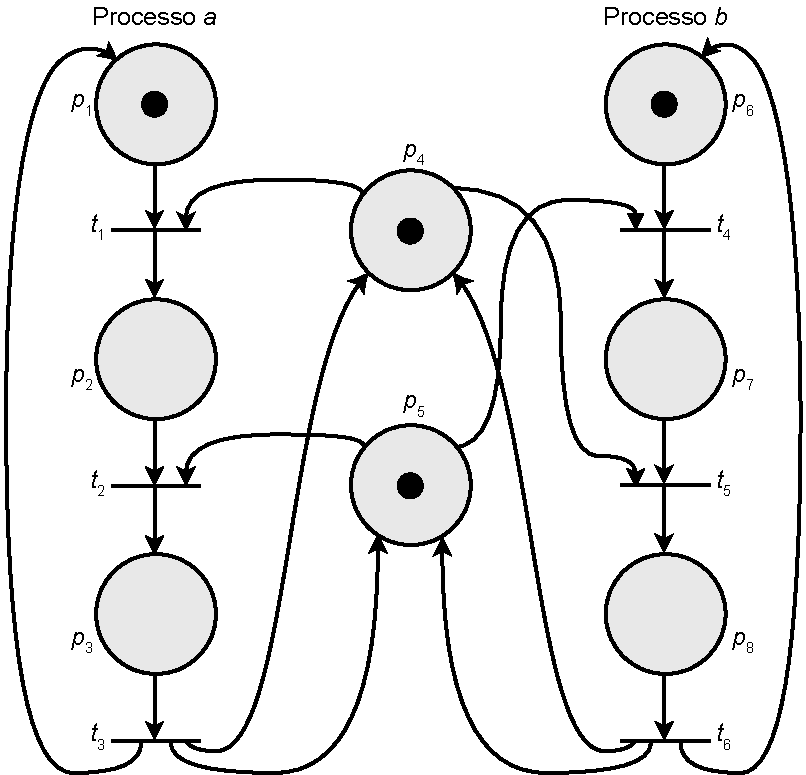
\includegraphics[width=0.7\textwidth]{resources/petri_net_peterson_deadlock}
	\end{center}
	\legend{Fonte: Adaptado de \citeonline[p. 86]{peterson:1981}}
\end{figure}



% \section{Modelagem de software}
% \label{sec:modelagem}
% \subsection{Transformações de modelo para código}